\documentclass{jlreq}

\usepackage{amsmath}
\usepackage{bm}
\usepackage{fancyhdr}
\usepackage{float}
\usepackage{graphicx}
\usepackage{physics}
\usepackage{siunitx}

\numberwithin{equation}{section}

\pagestyle{fancy}
\fancyhf{}
\fancyhead[R]{\thepage}

\begin{document}

\tableofcontents
\clearpage

\section{実験項目}
\begin{enumerate}
  \item 7400または74LS00のNANDゲートの入力電圧を0~5Vの範囲で変化させたとき,どのような出力が得られるかをオシロスコープを用いて観測する.
  \item 74HCU04のNOTゲートの伝達特性と消費電力特性に関して,入力電圧を0~5Vの範囲で変化させたときどのような出力が得られるかをオシロスコープを用いて測定する.
  \item 7400/74LS00を5個以上使って,それぞれをNOT素子として用いてリング発振器を構成し,その発振波形をオシロスコープで観測し,1素子当たりの平均遅延時間を求める.
\end{enumerate}

\section{目的}
\subsection{4週目}
いくつかのディジタルICを用いてNOTゲートの伝達特性や消費電力特性を調べ,TTLとCMOSの特性の違いを確認する.

\section{使用するソフトと部品}
\begin{itemize}
  \item Excel
  \item $68\si{\Omega}$の抵抗
  \item ジャンパーワイヤー
  \item ブレッドボード
  \item 74LS00 IC
  \item 74HCU04 IC
  \item Analog Discovery
  \item BNC Adapter
  \item WaveForms
\end{itemize}

\section{結果}
\subsection{実験1}
TTL素子は74LS00を用いた.NANDゲートの伝達特性の測定結果を表\ref{tab:io_feature}に示す.
\begin{table}[H]
  \centering
  \caption{74LS00のNANDゲートの伝達特性}
  \begin{tabular}{|r|r|}
    \hline
    入力電圧(V) & 出力電圧(V) \\ \hline
    0.00        & 4.34        \\ \hline
    0.50        & 4.10        \\ \hline
    0.80        & 3.90        \\ \hline
    1.00        & 3.16        \\ \hline
    1.50        & 0.13        \\ \hline
    2.00        & 0.13        \\ \hline
    2.51        & 0.13        \\ \hline
    5.03        & 0.13        \\ \hline
  \end{tabular}
  \label{tab:io_feature}
\end{table}

また,測定結果から得られたグラフを図\ref{fig:74LS00_io_feature}に示す.
\begin{figure}[H]
  \centering
  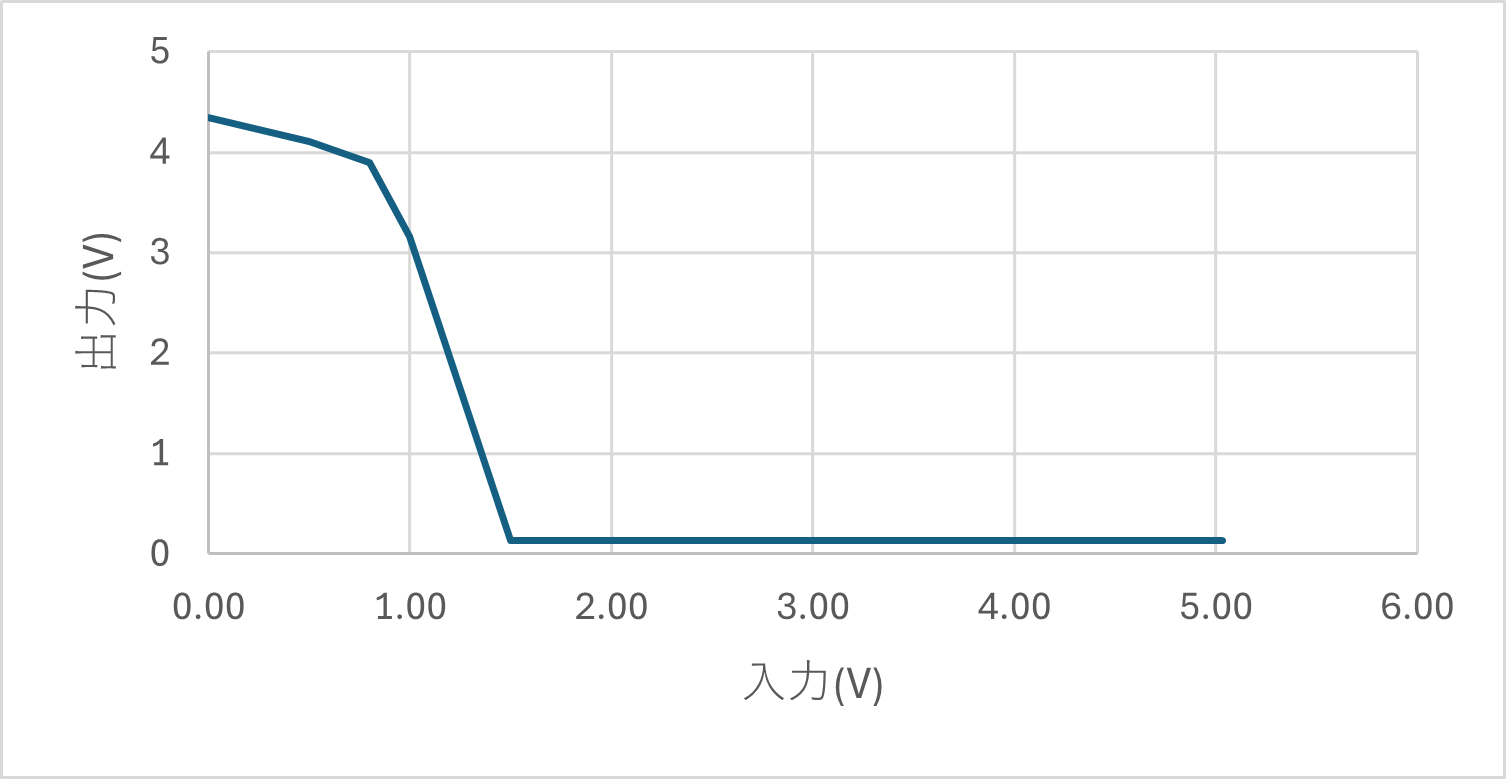
\includegraphics{assets/74LS00_io_feature.png}
  \caption{74LS00のNANDゲートの伝達特性のグラフ}
  \label{fig:74LS00_io_feature}
\end{figure}

\subsection{実験2}
TTL素子は74HCU04を用いた.NOTゲートの伝達特性を表\ref{tab:74HCU04_io_feature}に示す.
\begin{table}[H]
  \centering
  \caption{74HCU04のNOTゲートの伝達特性}
  \begin{tabular}{|r|r|}
    \hline
    入力電圧(V) & 出力電圧(V) \\ \hline
    0.00        & 4.97        \\ \hline
    0.49        & 4.97        \\ \hline
    1.00        & 4.95        \\ \hline
    1.50        & 4.85        \\ \hline
    2.01        & 4.56        \\ \hline
    2.51        & 3.39        \\ \hline
    3.02        & 0.44        \\ \hline
    3.52        & 0.13        \\ \hline
    5.04        & 0.01        \\ \hline
  \end{tabular}
  \label{tab:74HCU04_io_feature}
\end{table}

また,測定結果から得られたグラフを図\ref{fig:74HCU04_io_feature}に示す.
\begin{figure}[H]
  \centering
  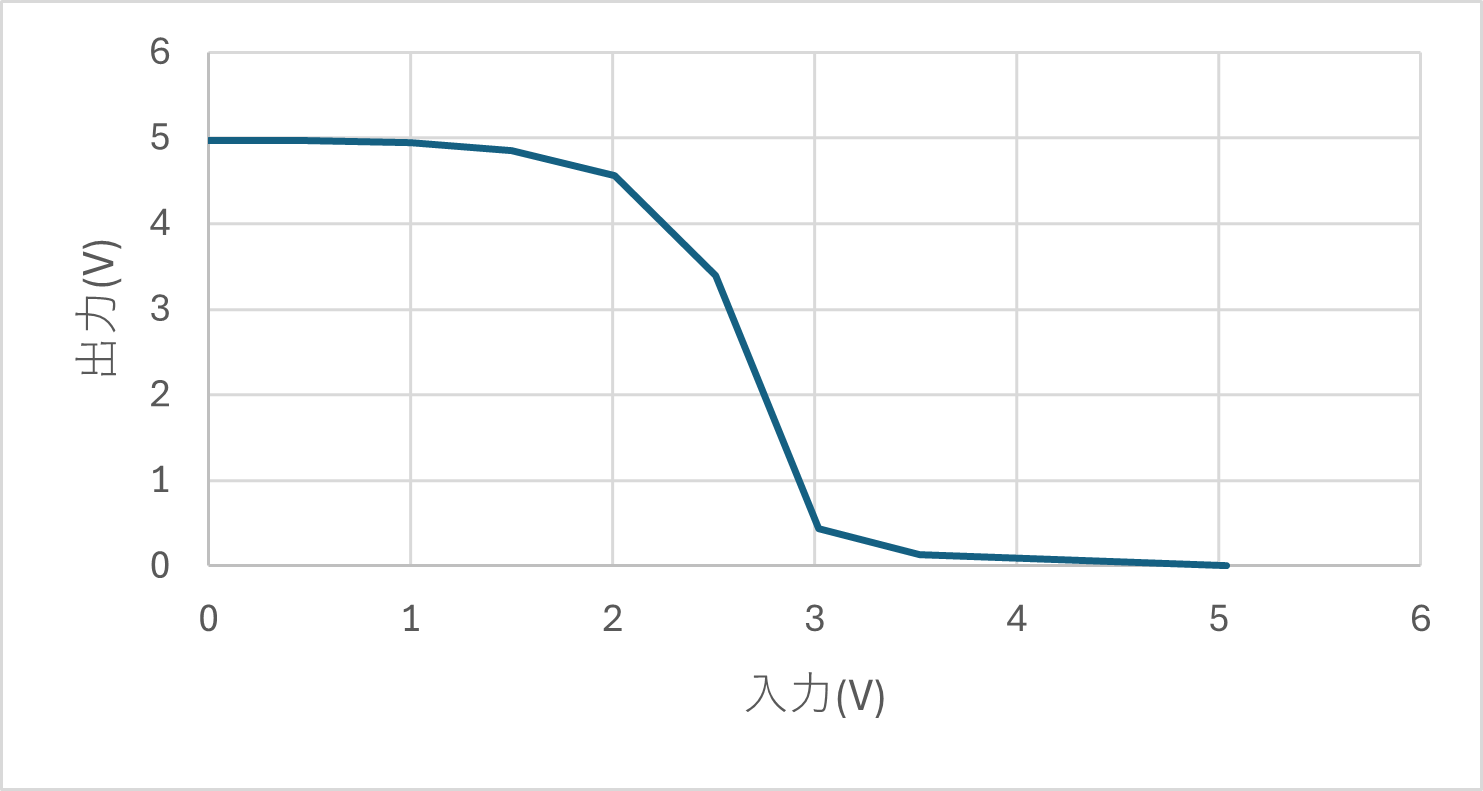
\includegraphics{assets/74HCU04_io_feature.png}
  \caption{74HCU04のNOTゲートの伝達特性のグラフ}
  \label{fig:74HCU04_io_feature}
\end{figure}

次に,消費電力特性のグラフを図\ref{fig:power_feature}に示す.電流の測定には$68\Omega$の抵抗を用いた.
\begin{figure}[H]
  \centering
  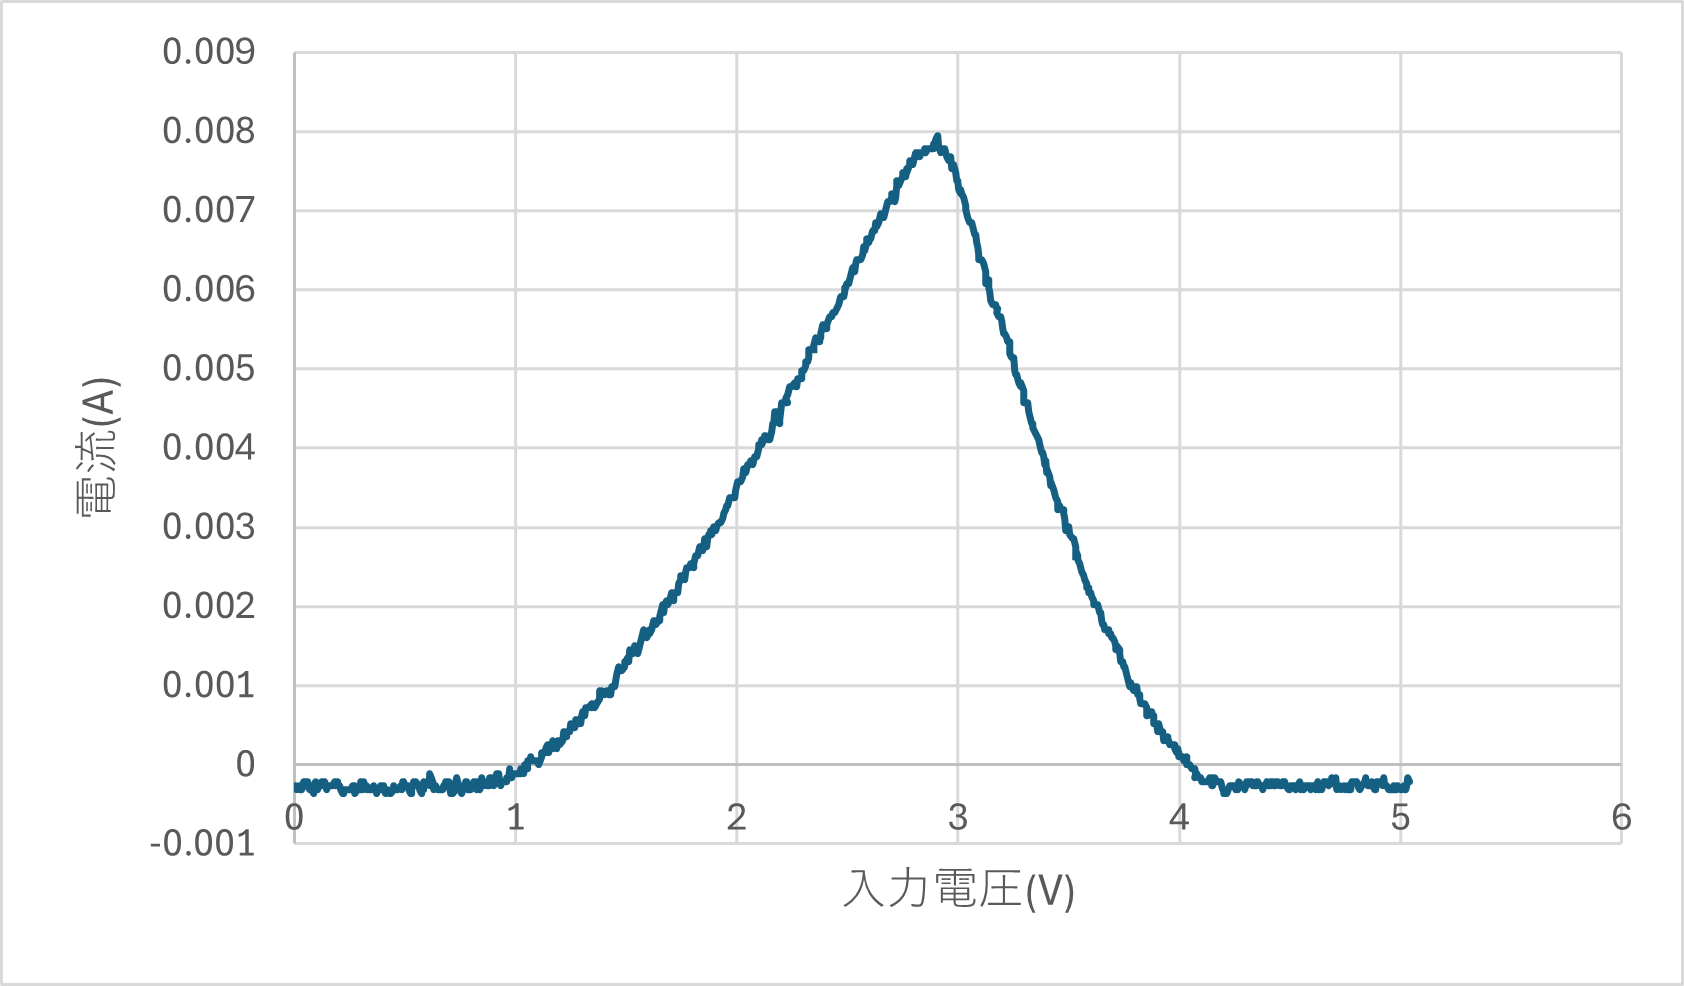
\includegraphics{assets/power_feature.png}
  \caption{74HCU04のNOTゲートの消費電力特性のグラフ}
  \label{fig:power_feature}
\end{figure}

\section{実験3}
リング発振器を構成する回路を組みTAからも確認を貰いながら測定を行ったところ,ブレッドボードの不具合か
素子の不具合か分からないが,うまく波形を出力することが出来なかったため,今回は割愛する.

\section{問題の解答}
\subsection{課題1}
Hレベル出力端子とHレベル入力端子が配線でつながれている場合を考える.もしも同レベルの電圧の範囲が同じだとすると,
Hレベル出力端子から配線を通る際の僅かな抵抗によって電圧降下が生じてしまい,Hレベル入力端子にてHと認識されなくなる可能性がある.
そのため,同レベルの入力電圧の範囲と出力電圧の範囲に差を作ることにより,信号伝達の保証を行っていると考えられる.

\subsection{課題2}
\subsubsection{7400と7400}
レベルに関係なく,出力電流に対して入力電流は$\frac{1}{10}$の電流が最低限必要なため,ファンアウト数は10である.

\subsubsection{7400と74LS00}
Hレベルでの接続では,出力電流に対して入力電流は$\frac{1}{20}$の電流が最低限必要なため,ファンアウト数は20である.
また,Lレベルでの接続も同じように考えると,ファンアウト数は40である.
これらより,レベルに関係なく回路に支障をきたさないゲート数は20個である.

\subsubsection{74LS00と7400}
Hレベルでの接続では,出力電流に対して入力電流は$\frac{1}{10}$の電流が最低限必要なため,ファンアウト数は10である.
また,Lレベルでの接続も同じように考えると,ファンアウト数は5である.
これらより,レベルに関係なく回路に支障をきたさないゲート数は5個である.

\subsubsection{74LS00と74LS00}
レベルに関係なく,出力電流に対して入力電流は$\frac{1}{20}$の電流が最低限必要なため,ファンアウト数は20である.

\subsection{課題3}
入力電圧が閾値電圧付近であるとき,NMOSとPMOSが同時に動作することにより,電源からグランドに電流が流れる.
このために,閾値付近で大きなピークをとる.

\subsection{課題4}
CMOSのファンアウト数が増えるにつれてキャパシタンスの合計も増加するが,キャパシタの電荷を放電/充電する際に遅延が生じるため,
キャパシタンスの合計が増えると伝搬遅延時間も増加する.そのため,許容ファンアウト数よりも多くのキャパシタを繋いでしまうと,
回路の応答速度が低下してしまい,適切な動作が保証されなくなってしまう.

\subsection{課題5}
理想的な回路の場合,奇数個のNOTを用いてリング発振器を作成すると,1つめのNOTの前がLとしたとき,1周したときにHとなり矛盾が生じてしまう.
しかし,リング発振器は発振する.これは,NOT素子によって電圧が変化する際に遅延が生じ,その遅延がNOT素子ごとに発生することで
自発的に発振するようになっている.

また,リング発振器の発振周期$T$とNOT素子の平均遅延時間$t_d$との関係は,NOT素子の個数をn(奇数)としたとき,
\begin{equation}
  T = 2nt_d
\end{equation}
と表せられる.

\section{考察}
\subsection{実験1}
\subsection{実験2}
\subsection{実験3}

\begin{thebibliography}{9}
  \item シリアーラヤ パノット.プロジェクト実習Ⅰ エレクトロニクス基礎 実験テキスト.京都工芸繊維大学,2024年
\end{thebibliography}

\end{document}